\documentclass[10pt,twocolumn,letterpaper]{article}

\usepackage{iccv}
\usepackage{times}
\usepackage{epsfig}
\usepackage{graphicx}
\usepackage{amsmath}
\usepackage{amssymb}
\usepackage{float}
% \usepackage{tikz}

% Include other packages here, before hyperref.

% egpaper.aux before re-running latex.  (Or just hit 'q' on the first latex
% run, let it finish, and you should be clear).
\usepackage[breaklinks=true,bookmarks=false]{hyperref}

\iccvfinalcopy % *** Uncomment this line for the final submission

\def\iccvPaperID{****} % *** Enter the ICCV Paper ID here
\def\httilde{\mbox{\tt\raisebox{-.5ex}{\symbol{126}}}}

% Pages are numbered in submission mode, and unnumbered in camera-ready
%\ificcvfinal\pagestyle{empty}\fi
\setcounter{page}{1}
\begin{document}

%%%%%%%%% TITLE
\title{Task Adaptation Strategies for Language Models}

\author{Anmol Agarwal\\
	Georgia Institute of Technology\\
	{\tt\small aagarwal622@gatech.edu}
	% For a paper whose authors are all at the same institution,
	% omit the following lines up until the closing ``}''.
	% Additional authors and addresses can be added with ``\and'',
	% just like the second author.
	% To save space, use either the email address or home page, not both
	\and
	Rayyan Shahid\\
	Georgia Institute of Technology\\
	{\tt\small rshahid9@gatech.edu}
}

\maketitle
%\thispagestyle{empty}

% FROM blang/latex

% RUN apt-get update && apt-get install -y biber


%%%%%%%%% ABSTRACT
\begin{abstract}
	Large Language Models (LLMs) have demonstrated remarkable performance across various language tasks, yet achieving optimal performance often requires task-specific adaptation. This paper delves into the comparative analysis of several adaptation strategies, focusing on Few-Shot Fine Tuning, In-Context Learning, and Context Distillation. Additionally, it introduces two novel strategies: In-Context Learning with Few-Shot Fine Tuning and Context Distillation with Few-Shot Fine Tuning. The study evaluates these strategies on the NLI task using models from the OPT family, measuring both in-domain and out-of-domain accuracies. Results indicate that Few-Shot Fine Tuning consistently outperforms other strategies across various model sizes, demonstrating superior in-domain and out-of-domain generalization, along with a higher sample processing rate. These findings underscore the effectiveness of Few-Shot Fine Tuning as the preferred task adaptation strategy for the NLI task on the OPT family of models, potentially enhancing the capabilities of existing LLMs without extensive re-training or fine-tuning on large datasets.\\\\
\end{abstract}
\href{https://github.com/sicario001/llmft}{\textbf{Project GitHub repository}}\\
\href{https://github.com/sicario001/llmft}{https://github.com/sicario001/llmft}

%%%%%%%%% BODY TEXT
\begin{table*}[h!]
\begin{center}
\begin{tabular}{|c|c|c|c|c|}
\hline
\textbf{Seed} & \textbf{Train Accuracy} & \textbf{MNLI Eval} & \textbf{HANS Entail} & \textbf{HANS Contradict} \\
\hline
\hline
0 & 0.48 & 0.528 & 1 & 0 \\
1 & 0.49 & 0.5204 & 1 & 0 \\
2 & 0.49 & 0.5248 & 1 & 0 \\
3 & 0.5 & 0.5289 & 1 & 0 \\
4 & 0.49 & 0.5225 & 1 & 0 \\
\hline
\end{tabular}
\end{center}
\caption{Accuracy for In-Context Learning (A1) for OPT-125m model}
\end{table*}

% Add a table for accuracies for approach A1 for opt-1.3b
% opt-1.3b	accuracy			
% Seed	Train Accuracy	mnli-eval	hans-entail	hans-contradict
% 0	0.69	0.6096	0.1846	0.791
% 1	0.63	0.6279	0.7176	0.3126
% 2	0.59	0.5487	0.0136	0.9876
% 3	0.69	0.6304	0.554	0.4786
% 4	0.59	0.6087	0.5136	0.4248

\begin{table*}[h!]
\begin{center}
\begin{tabular}{|c|c|c|c|c|}
\hline
\textbf{Seed} & \textbf{Train Accuracy} & \textbf{MNLI Eval} & \textbf{HANS Entail} & \textbf{HANS Contradict} \\
\hline
\hline
0 & 0.69 & 0.6096 & 0.1846 & 0.791 \\
1 & 0.63 & 0.6279 & 0.7176 & 0.3126 \\
2 & 0.59 & 0.5487 & 0.0136 & 0.9876 \\
3 & 0.69 & 0.6304 & 0.554 & 0.4786 \\
4 & 0.59 & 0.6087 & 0.5136 & 0.4248 \\
\hline
\end{tabular}
\end{center}
\caption{Accuracy for In-Context Learning (A1) for OPT-1.3b model}
\end{table*}

	

\section{Introduction/Background/Motivation}
In recent years, Large Language Models (LLMs) have shown great performance across various language tasks. However, the models need to be adapted to the specific task in consideration to extract the best possible performance. There are several different adaptation strategies. Two common ones include: \textit{few-shot fine tuning} and \textit{in-context learning (ICL)}. \cite {mosbach2023fewshot} explores these two adaptation strategies in detail and offers a fair comparison between the two. They compare models of different sizes from the OPT and Pythia family for different context lengths on datasets like RTE, MNLI and QQP by measuring both in-domain and out-of-domain accuracies. They conclude that unlike the earlier belief that in-context learning greatly outperforms few-shot fine tuning, if we fairly compare the two strategies, the results are much closer and generally in favor of few-shot fine tuning. Moreover, few-shot fine tuning has an added benefit of reduced runtime latency and correspondingly higher sample processing rate as compared in-context learning because of smaller context sizes at the time of inference. \cite{askell2021general} explores a different context-distillation based fine tuning strategy for Language Models. This differs from few-shot finetuning and in-context learning strategies in the fact that apart from using a few high quality labelled samples as the context, it also utilizes a large unlabelled training dataset for fine tuning the model. It has the same benefits in terms of runtime latency as few-shot fine tuning because it doesn't require contexts to be provided at inference time.

In this work, we compare the above task adaptation strategies i.e few-shot fine tuning, in-context learning and context distillation, and also propose two new task adaptation strategies - namely in-context learning with few-shot fine tuning and context distillation with few-shot fine tuning. The motivation behind using in-context learning with few-shot fine tuning is that it allows the model to leverage the context data through both the strategies. The motivation behind using context distillation with few-shot fine tuning is that it should in theory provide the performance of in-context learning with few-shot fine tuning while also providing the runtime latency benefits of context distillation because of the absence of context at inference time. 

If this project proves successful, it could significantly enhance the capabilities of existing Large Language Models (LLMs). This would enable them to handle extended dialogue conversations more effectively, answer queries about extensive PDF files, or even auto-complete code while being aware of a large repository. All these improvements could be achieved without the necessity for costly re-training from the ground up or fine-tuning on extensive datasets.


We will describe each of the above strategies in detail in the following section. We will also provide evaluation results for the above strategies for the OPT family on the MNLI dataset for different context lengths. We also report out-of-domain generalization results on the lexical overlap subset of HANS dataset. Please refer to the experimental setup section for more details on the datasets and evaluation metrics used.

\section{Approach}
% A2 
% opt-125m	accuracy		
% Seed	mnli-eval	hans-entail	hans-contradict
% 0	0.5766	1	0
% 1	0.598	0.9526	0.0276
% 2	0.5372	1	0
% 3	0.556	0.105	0.9006
% 4	0.6462	1	0
		
		
% opt-1.3b	accuracy		
% Seed	mnli-eval	hans-entail	hans-contradict
% 0	0.6827	0.8878	0.145
% 1	0.6573	0.9244	0.1204
% 2	0.579	1	0
% 3	0.6918	0.5916	0.4918
% 4	0.6649	1	0

\begin{table*}[h!]
\begin{center}
\begin{tabular}{|c|c|c|c|c|}
\hline
\textbf{Seed} & \textbf{MNLI Eval} & \textbf{HANS Entail} & \textbf{HANS Contradict} \\
\hline
\hline
0 & 0.5766 & 1 & 0 \\
1 & 0.598 & 0.9526 & 0.0276 \\
2 & 0.5372 & 1 & 0 \\
3 & 0.556 & 0.105 & 0.9006 \\
4 & 0.6462 & 1 & 0 \\
\hline
\end{tabular}
\end{center}
\caption{Accuracy for Few-Shot Fine Tuning (A2) for OPT-125m model}
\end{table*}

\begin{table*}[h!]
\begin{center}
\begin{tabular}{|c|c|c|c|c|}
\hline
\textbf{Seed} & \textbf{MNLI Eval} & \textbf{HANS Entail} & \textbf{HANS Contradict} \\
\hline
\hline
0 & 0.6827 & 0.8878 & 0.145 \\
1 & 0.6573 & 0.9244 & 0.1204 \\
2 & 0.579 & 1 & 0 \\
3 & 0.6918 & 0.5916 & 0.4918 \\
4 & 0.6649 & 1 & 0 \\
\hline
\end{tabular}
\end{center}
\caption{Accuracy for Few-Shot Fine Tuning (A2) for OPT-1.3b model}
\end{table*}


In this section, we will describe the approach for the different task adaptation strategies explored as part of this work. This includes three existing task adaptation strategies:
\begin{enumerate}
    \item In-Context Learning (\textbf{A1})
	\item Few-Shot Fine Tuning (\textbf{A2})
	\item Context Distillation (\textbf{A3})
\end{enumerate}
We also propose two new task adaptation strategies:
\begin{enumerate}
	\item In-Context Learning with Few-Shot Fine Tuning (\textbf{A4})
	\item Context Distillation with Few-Shot Fine Tuning (\textbf{A5})
\end{enumerate}
Apart from the labelled context data, the context distillation based approaches also rely on an unlabelled dataset that would be used for fine tuning the language model based on a distillation loss with respect to a reference model. 
\subsection{In-Context Learning}
In-context learning is an approach in which model is given context containing a fixed number of examples for a task with expected output, and then model is given a 
new example for which the model has to generate an output based on the context. \\
For example:
% TODO: format this example properly in latex
\begin{verbatim}
Question 1: What is the capital of UK?
Answer 1: Paris
Correct: No
        
Question 2: What is the capital of India?
Answer 2: Berlin
Correct: No
        
Question 3: What is the capital of Italy?
Answer 3: Rome
Correct: Yes
        
Question 4: What is the capital of Spain?
Answer 4: Amsterdam
Correct: ?
\end{verbatim}
In the above output, the model is given context containing 3 examples and their expected outputs. The model is then asked to predict the output for the 4th example. The model is then evaluated based on the correctness of the output for the 4th example. \\
One drawback of in-context learning is large context length, as the context length increases, the model becomes slower and has to remember more context.

\subsection{Few-Shot Fine Tuning}
In few-shot fine-tuning, the model is given a few examples for a task with expected output, and then the model is fine-tuned on these examples. The model is then evaluated on a new example for which the model has to generate an output. \\
This approach may be better than in-context learning from the perspective of model speed and memory usage, as the model only has to process one example rather than entire context.

\subsection{Context Distillation}
Here we have two pretrained models. One model is given context as input, and it has to generate an output for a new example based on the context.
We also have another model (initially similar to the first one) which fine tunes on labels generated by first model.
In other words, second model is fine tuned on the unlabelled dataset using a distillation loss with respect to the first model.\\
Let $X$ be unlabeled dataset, $C$ be the context provided to first model to infer the output. This approach is different because few-shot 
fine-tuning models the distribution $P(X)$ and in-context learning models the distribution $P(X|C)$.
We instead want the fine-tuned model to model the distribution $P(X|C)$ despite being given no context. Context distillation helps in achieving this.
The first model models the distribution $P(X|C)$ and the second model models the distribution $P(X)$.
And our goal is to minimize the KL divergence between the two distributions.\\
The distillation loss is given by:
\begin{equation}
	L_{distillation}(\theta) = KL(P_0(X|C) || P_{\theta}(X))
\end{equation}
Where $P_0(X|C)$ is the distribution modeled by the first model and $P_{\theta}(X)$ is the distribution modeled by the second model. Through this
loss, the second model learns to model the distribution $P(X|C)$ despite being given no context.

\subsection{In-Context Learning with Few-Shot Fine Tuning}
Since it was shown in <cite> paper that fine-tuning can perform better than in-context learning, we wanted to see if fine-tuned model is given context,
will it perform better than in-context learning with pretrained model.
In this approach, first model is fine-tuned on few examples and then given context as input to generate output for a new example.\\
Intuitively speaking, we wanted to validate the hypothesis that since fine-tuned model has already seen examples and being slightly adapted to the task, it might be able to generate better output
for the new example given context than the pretrained model.

\subsection{Context Distillation with Few-Shot Fine Tuning}
In this approach, we wanted to see if context distillation can be used in conjunction with few-shot fine-tuning to improve the performance of the model due to the same reasons as
in the previous approach. Here, unlike vanilla context distillation, first model used is a fine-tuned one instead of being pretrained. The second model is still pretrained.

% A3
% Context Size 32			
% opt-125m	accuracy		
% Seed	mnli-eval	hans-entail	hans-contradict
% 3	0.52	1	0
		
		
		
		
		
		
% opt-1.3b	accuracy		
% Seed	mnli-eval	hans-entail	hans-contradict
% 3	0.6784	0.889	0.1204

\begin{table*}[h!]
\begin{center}
\begin{tabular}{|c|c|c|c|c|}
\hline
\textbf{Seed} & \textbf{MNLI Eval} & \textbf{HANS Entail} & \textbf{HANS Contradict} \\
\hline
\hline
3 & 0.52 & 1 & 0 \\
\hline
\end{tabular}
\end{center}
\caption{Accuracy for Context Distillation (A3) for OPT-125m model}
\end{table*}

\begin{table*}[h!]
\begin{center}
\begin{tabular}{|c|c|c|c|c|}
\hline
\textbf{Seed} & \textbf{MNLI Eval} & \textbf{HANS Entail} & \textbf{HANS Contradict} \\
\hline
\hline
3 & 0.6784 & 0.889 & 0.1204 \\
\hline
\end{tabular}
\end{center}
\caption{Accuracy for Context Distillation (A3) for OPT-1.3b model}
\end{table*}

% A4
% opt-125m	accuracy			
% Seed	Train Accuracy	mnli-eval	hans-entail	hans-contradict
% 0	0.49	0.5231	1	0
% 1	0.51	0.5309	1	0
% 2	0.49	0.5198	1	0
% 3	0.51	0.4801	0	1
% 4	0.57	0.5554	1	0
			
			
% opt-1.3b	accuracy			
% Seed	Train Accuracy	mnli-eval	hans-entail	hans-contradict
% 0	0.62	0.6256	0.9386	0.0526
% 1	0.53	0.5406	0.9986	0.0004
% 2	0.54	0.544	1	0
% 3	0.66	0.6531	0.8486	0.1484
% 4	0.66	0.6409	0.9496	0.042

\begin{table*}[h!]
\begin{center}
\begin{tabular}{|c|c|c|c|c|}
\hline
\textbf{Seed} & \textbf{Train Accuracy} & \textbf{MNLI Eval} & \textbf{HANS Entail} & \textbf{HANS Contradict} \\
\hline
\hline
0 & 0.49 & 0.5231 & 1 & 0 \\
1 & 0.51 & 0.5309 & 1 & 0 \\
2 & 0.49 & 0.5198 & 1 & 0 \\
3 & 0.51 & 0.4801 & 0 & 1 \\
4 & 0.57 & 0.5554 & 1 & 0 \\
\hline
\end{tabular}
\end{center}
\caption{Accuracy for In-Context Learning with Few-Shot Fine Tuning (A4) for OPT-125m model}
\end{table*}

\begin{table*}[h!]
\begin{center}
\begin{tabular}{|c|c|c|c|c|}
\hline
\textbf{Seed} & \textbf{Train Accuracy} & \textbf{MNLI Eval} & \textbf{HANS Entail} & \textbf{HANS Contradict} \\
\hline
\hline
0 & 0.62 & 0.6256 & 0.9386 & 0.0526 \\
1 & 0.53 & 0.5406 & 0.9986 & 0.0004 \\
2 & 0.54 & 0.544 & 1 & 0 \\
3 & 0.66 & 0.6531 & 0.8486 & 0.1484 \\
4 & 0.66 & 0.6409 & 0.9496 & 0.042 \\
\hline
\end{tabular}
\end{center}
\caption{Accuracy for In-Context Learning with Few-Shot Fine Tuning (A4) for OPT-1.3b model}
\end{table*}

% A5
% opt-125m	accuracy		
% Seed	mnli-eval	hans-entail	hans-contradict
% 3	0.5261	1	0
		
		
		
		
		
		
% opt-1.3b	accuracy		
% Seed	mnli-eval	hans-entail	hans-contradict
% 3	0.6672	0.9342	0.0794

\begin{table*}[h!]
	\begin{center}
	\begin{tabular}{|c|c|c|c|c|}
	\hline
	\textbf{Seed} & \textbf{MNLI Eval} & \textbf{HANS Entail} & \textbf{HANS Contradict} \\
	\hline
	\hline
	3 & 0.5261 & 1 & 0 \\
	\hline
	\end{tabular}
	\end{center}
	\caption{Accuracy for Context Distillation with Few-Shot Fine Tuning (A5) for OPT-125m model}
	\end{table*}
	
	\begin{table*}[h!]
	\begin{center}
	\begin{tabular}{|c|c|c|c|c|}
	\hline
	\textbf{Seed} & \textbf{MNLI Eval} & \textbf{HANS Entail} & \textbf{HANS Contradict} \\
	\hline
	\hline
	3 & 0.6672 & 0.9342 & 0.0794 \\
	\hline
	\end{tabular}
	\end{center}
	\caption{Accuracy for Context Distillation with Few-Shot Fine Tuning (A5) for OPT-1.3b model}
	\end{table*}

\section{Experimental Setup}
We compute the performance of the above task adaptation strategies focusing on in-domain and out-of-domain generalization for the natural language inference (NLI) task.\\
\textbf{Model} We choose the OPT model family and specifically the OPT-125m and OPT-1.3b models.\\
\textbf{Datasets} We use the MNLI training dataset for generating the context data. For in-domain generalization, we use the validation set of MNLI dataset. For out-of-domain generalization, we choose the lexical overlap subset of HANS. The MNLI dataset is binarized by removing the neutral samples.\\
\textbf{Evaluation Metrics} We use the following evaluation metrics
\footnote{Out-of-domain accuracy is computed as the mean of accuracies of HANS-Lexical\_overlap-entailment and HANS-Lexical\_overlap-contradiction.}
\begin{itemize}
    \item Accuracy on MNLI validation dataset
    \item Accuracy on HANS-Lexical\_overlap-entailment
    \item Accuracy on HANS-Lexical\_overlap-contradiction
    \item Samples processed per second
\end{itemize}
\textbf{Context Size} We evaluate the training strategies on a context size of 32. For in-context leanrning based strategies, this means providing a context of 32 examples during evaluation. For few-shot fine tuning based strategies, this means providing 32 examples for fine-tuning the model. For context distillation, we randomly sample a subset of 100 examples from the binarized MNLI training dataset and remove their ground-truth labels. The models are then fine tuned using a distillation loss against a reference moodel.\\
\textbf{Seeds} We use 5 different seeds for choosing a random context of 32 examples for each of the following strategies-
\begin{enumerate}
    \item In-Context Learning
    \item Few-Shot Fine Tuning
    \item In-Context Learning with Few-Shot Fine Tuning
\end{enumerate}
For Context Distillation, we use the best performing seed from the In-Context Learning strategy. For Context Distillation with Few-Shot Fine Tuning, we use the best performing seed from the In-Context Learning with Few-Shot Fine Tuning strategy.\\

For the fine tuning based strategies, we fine tune the model for 40 epochs with a batch size of 4.\\\\
Our training and evaluation was run on a VM with NVIDIA RTX A6000 48 GB GPU, 2 AMD EPYC 7282 vCPUs and 48 GB RAM.


	

\newpage
\section{Results and Discussion}
% Insert figure figures/opt_125m-accuracy.png
% Insert figure figures/opt_1.3b-accuracy.png

\begin{figure}[h]
\begin{center}
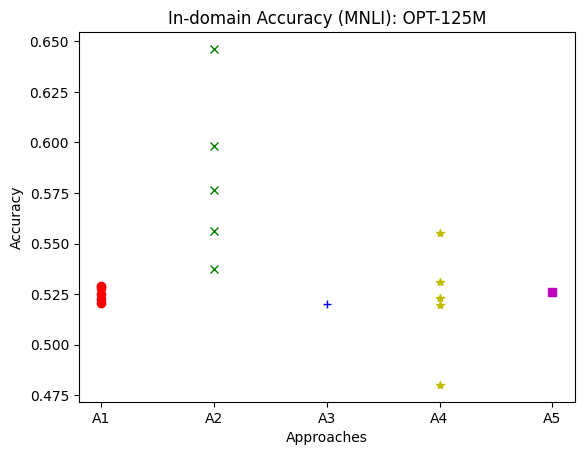
\includegraphics[width=0.8\linewidth]{figures/opt-125m-accuracy.png}
\end{center}
\caption{Accuracy on MNLI validation dataset for OPT-125m model}
\end{figure}

\begin{figure}[h]
\begin{center}
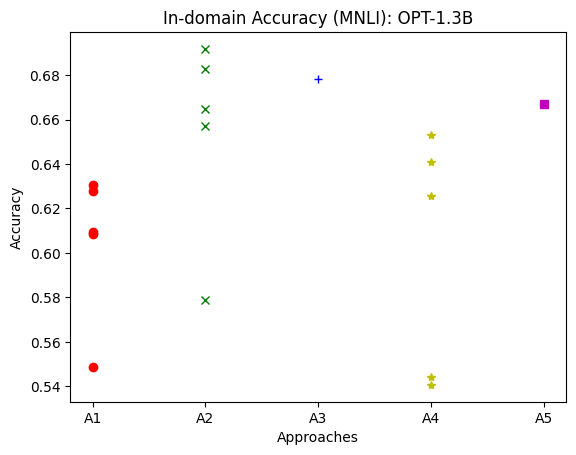
\includegraphics[width=0.8\linewidth]{figures/opt-1_3b-accuracy.png}
\end{center}
\caption{Accuracy on MNLI validation dataset for OPT-1.3b model}
\end{figure}

% Out of domain accuracy on HANS
% Insert figure figures/hans-accuracy.png
\begin{figure}[h]
\begin{center}
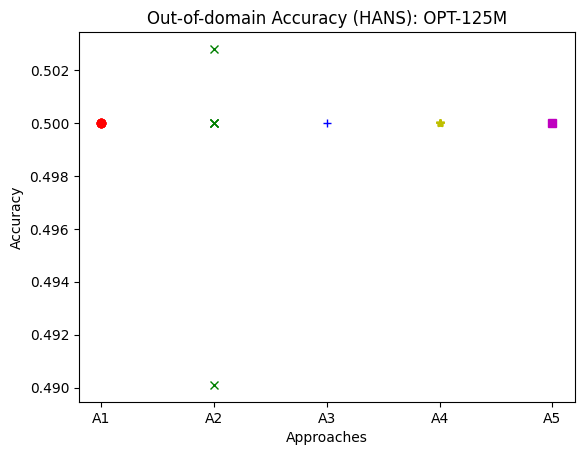
\includegraphics[width=0.8\linewidth]{figures/out-of-domain-opt-125m.png}
\end{center}
\caption{Out of domain accuracy on HANS dataset for OPT-125m}
\end{figure}

\begin{figure}[h]
    \begin{center}
    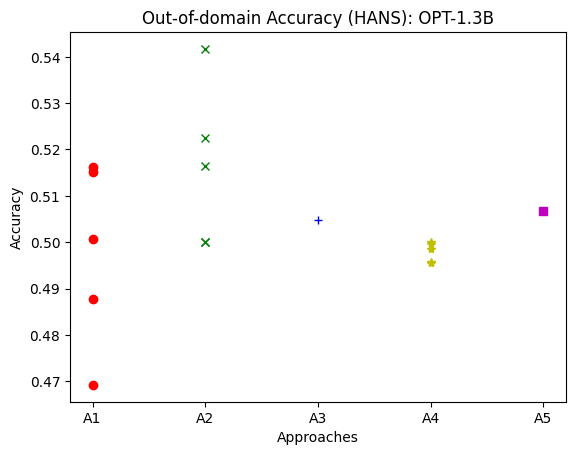
\includegraphics[width=0.8\linewidth]{figures/out-of-domain-opt-1_3b.png}
    \end{center}
    \caption{Out of domain accuracy on HANS dataset for OPT-1.3B}
    \end{figure}
    

% Insert figures sample rates
\begin{figure}[h]
\begin{center}
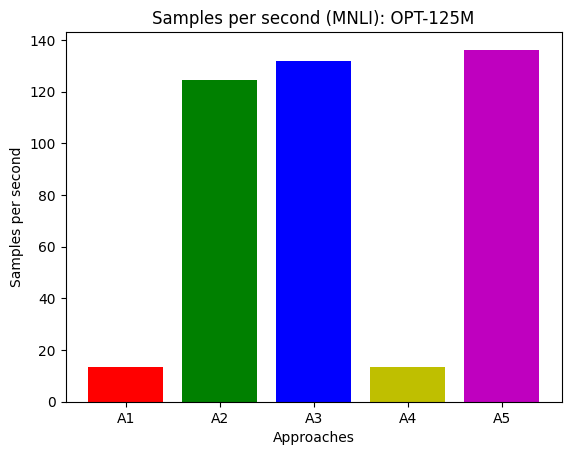
\includegraphics[width=0.8\linewidth]{figures/samples-opt125m.png}
\end{center}
\caption{Samples processed per second for OPT-125m model}
\end{figure}

\begin{figure}[H]
\begin{center}
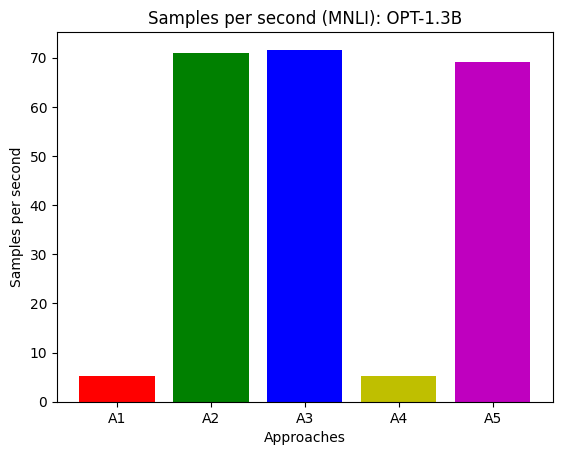
\includegraphics[width=0.8\linewidth]{figures/samples-opt1_3B.png}
\end{center}
\caption{Samples processed per second for OPT-1.3B model}
\end{figure}

% Based on figure 1, for opt-125m, A2 i.e few-shot fine tuning achieves the best in-domain performance across the 5 enalyzed strategies on the NLI task. A4 i.e in-context learning with few-shot fine tuning achieves the second best performance. The other strategies i.e A1, A3 and A4 perform close to each other.
% Based on figure 2, for opt1.3b, A2 again achieves best in domain accuracy. The order of accuracies in this case is A2 > A3 > A5 > A4 > A1.

Based on figure 1, for OPT-125m, Few-Shot Fine Tuning (A2) achieves the best in-domain performance across the 5 analyzed strategies on the NLI task. In-Context Learning with Few-Shot Fine Tuning (A4) achieves the second best performance. The other strategies i.e In-Context Learning (A1), Context Distillation (A3) and Context Distillation with Few-Shot Fine Tuning (A5) perform close to each other.\\

Based on figure 2, for OPT-1.3b, Few-Shot Fine Tuning (A2) again achieves the best in-domain accuracy. The order of accuracies in this case is A2 $>$ A3 $>$ A5 $>$ A4 $>$ A1.\\


% Based on figure 3, for opt-125m, A2 achieves the best out of domain accuracy. The other strategies have a similar performance. For opt-1.3b, A2 again achieves the best out of domain accuracy. sURPRISINGLY, A4 has the worst out of domain accuracy (max across seeds) for opt-1.3b.

Based on figure 3, for OPT-125m, Few-Shot Fine Tuning (A2) achieves the best out of domain accuracy. The other strategies have a similar performance. For OPT-1.3b, Few-Shot Fine Tuning (A2) again achieves the best out of domain accuracy. Surprisingly, In-Context Learning with Few-Shot Fine Tuning (A4) has the worst out of domain accuracy (max across seeds) for OPT-1.3b.\\

% Based on figure 4 and 5, A2, A3 and A5 have similar samples processing rate. A1 and A4 have a lower samples processing rate. This is consistent with our expectations as A1 and A4 require context at inference time which increases the latency.

Based on figure 4 and 5, Few-Shot Fine Tuning (A2), Context Distillation (A3) and Context Distillation with Few-Shot Fine Tuning (A5) have similar samples processing rate. In-Context Learning (A1) and In-Context Learning with Few-Shot Fine Tuning (A4) have a lower samples processing rate. This is consistent with our expectations as A1 and A4 require context at inference time which increases the latency.\\

% Overall, A2 i.e few-shot fine tuning performs the best for both in-domain and out-of-domain generalization as well as sample processing rate. Therefpre, we can conclude that few-shot fine tuning is the best task adaptation strategy among the tested strategies for the NLI task on the OPT family of models based on the experiments conducted in this work.

Overall, Few-Shot Fine Tuning (A2) performs the best for both in-domain and out-of-domain generalization as well as sample processing rate. Therefore, we can conclude that few-shot fine tuning is the best task adaptation strategy among the tested strategies for the NLI task on the OPT family of models based on the experiments conducted in this work.






\section{Challenges}
\begin{enumerate}
    \item \textbf{Resource Constraints:} The larger models in the OPT family (for eg. OPT-30b) require a large amount of GPU memory and training time. Because of our resouce and cost constrainsts, we were unable to evaluate these models. We also had to fix the context size to 32 examples and could only run the experiment for 5 seeds for non context-distillation based approaches. Our experiments on an RTX A6000 48 GB GPU were limited to the OPT-125m and OPT-1.3b models for the NLI task and took a total of \$60 spanned over a week.
    \item \textbf{Environment Setup:} The existing codebase for llmft utilized a docker container for environment setup. This was not possible to setup on PACE VMs. As a result, we had to setup our development environemnt locally and run the experiments on GPUs reserved over tensordock.  
    %Only evaluated for NLI task using MNLI dataset. Could have been more comprehensive. Due to time constraints 
    \item \textbf{Datasets:} Because of time and cost constraints, we only evaluated the strategies for the NLI task on the MNLI and lexical overlap of HANS datasets. Evaluating the models on more datasets would have given us a better understanding of the generalization capabilities of these task adaptation strategies.
\end{enumerate}
\section{Work Division}
% Create a student contributions table and use checkmarks to indicate who did what
%define checkmark


\begin{table}[h!]
\begin{center}
\begin{tabular}{|c|c|c|}
\hline
\textbf{Task} & \textbf{Anmol} & \textbf{Rayyan} \\
\hline
\hline
\textbf{A1 experiments} & \checkmark & \\
\hline
\textbf{A2 experiments} & \checkmark & \\
\hline
\textbf{A3 code} & & \checkmark \\
\hline
\textbf{A3 experiments} & & \checkmark\\
\hline
\textbf{A4 code} & \checkmark & \\
\hline
\textbf{A4 experiments} & \checkmark & \\
\hline
\textbf{A5 code} & &\checkmark \\
\hline
\textbf{A5 experiments} & & \checkmark\\
\hline
\textbf{Report} & \checkmark & \checkmark\\
\hline
\end{tabular}
\end{center}
\caption{Student Contributions}
\end{table}

%-------------------------------------------------------------------------
% \subsection{Language}

% All manuscripts must be in English.

% \subsection{Dual submission}

% Please refer to the author guidelines on the ICCV 2017 web page for a
% discussion of the policy on dual submissions.

% \subsection{Paper length}
% For ICCV 2017, the rules about paper length have changed, so please
% read this section carefully. Papers, excluding the references section,
% must be no longer than eight pages in length. One additional page 
% containing {\em only} cited references is allowed, for a total maximal 
% length of nine pages. 


% Overlength papers will simply not be reviewed.  This includes papers
% where the margins and formatting are deemed to have been significantly
% altered from those laid down by this style guide.  Note that this
% \LaTeX\ guide already sets figure captions and references in a smaller font.
% The reason such papers will not be reviewed is that there is no provision for
% supervised revisions of manuscripts.  The reviewing process cannot determine
% the suitability of the paper for presentation in eight pages if it is
% reviewed in eleven.  

% %-------------------------------------------------------------------------
% \subsection{The ruler}
% The \LaTeX\ style defines a printed ruler which should be present in the
% version submitted for review.  The ruler is provided in order that
% reviewers may comment on particular lines in the paper without
% circumlocution.  If you are preparing a document using a non-\LaTeX\
% document preparation system, please arrange for an equivalent ruler to
% appear on the final output pages.  The presence or absence of the ruler
% should not change the appearance of any other content on the page.  The
% camera ready copy should not contain a ruler. (\LaTeX\ users may uncomment
% the \verb'\iccvfinalcopy' command in the document preamble.)  Reviewers:
% note that the ruler measurements do not align well with lines in the paper
% --- this turns out to be very difficult to do well when the paper contains
% many figures and equations, and, when done, looks ugly.  Just use fractional
% references (e.g.\ this line is $095.5$), although in most cases one would
% expect that the approximate location will be adequate.

% \subsection{Mathematics}

% Please number all of your sections and displayed equations.  It is
% important for readers to be able to refer to any particular equation.  Just
% because you didn't refer to it in the text doesn't mean some future reader
% might not need to refer to it.  It is cumbersome to have to use
% circumlocutions like ``the equation second from the top of page 3 column
% 1''.  (Note that the ruler will not be present in the final copy, so is not
% an alternative to equation numbers).  All authors will benefit from reading
% Mermin's description of how to write mathematics:
% \url{http://www.pamitc.org/documents/mermin.pdf}.


% \subsection{Blind review}

% Many authors misunderstand the concept of anonymizing for blind
% review.  Blind review does not mean that one must remove
% citations to one's own work---in fact it is often impossible to
% review a paper unless the previous citations are known and
% available.

% Blind review means that you do not use the words ``my'' or ``our''
% when citing previous work.  That is all.  (But see below for
% techreports.)

% Saying ``this builds on the work of Lucy Smith [1]'' does not say
% that you are Lucy Smith; it says that you are building on her
% work.  If you are Smith and Jones, do not say ``as we show in
% [7]'', say ``as Smith and Jones show in [7]'' and at the end of the
% paper, include reference 7 as you would any other cited work.

% An example of a bad paper just asking to be rejected:
% \begin{quote}
% \begin{center}
%     An analysis of the frobnicatable foo filter.
% \end{center}

%    In this paper we present a performance analysis of our
%    previous paper [1], and show it to be inferior to all
%    previously known methods.  Why the previous paper was
%    accepted without this analysis is beyond me.

%    [1] Removed for blind review
% \end{quote}


% An example of an acceptable paper:

% \begin{quote}
% \begin{center}
%      An analysis of the frobnicatable foo filter.
% \end{center}

%    In this paper we present a performance analysis of the
%    paper of Smith \etal [1], and show it to be inferior to
%    all previously known methods.  Why the previous paper
%    was accepted without this analysis is beyond me.

%    [1] Smith, L and Jones, C. ``The frobnicatable foo
%    filter, a fundamental contribution to human knowledge''.
%    Nature 381(12), 1-213.
% \end{quote}

% If you are making a submission to another conference at the same time,
% which covers similar or overlapping material, you may need to refer to that
% submission in order to explain the differences, just as you would if you
% had previously published related work.  In such cases, include the
% anonymized parallel submission~\cite{Authors14} as additional material and
% cite it as
% \begin{quote}
% [1] Authors. ``The frobnicatable foo filter'', F\&G 2014 Submission ID 324,
% Supplied as additional material {\tt fg324.pdf}.
% \end{quote}

% Finally, you may feel you need to tell the reader that more details can be
% found elsewhere, and refer them to a technical report.  For conference
% submissions, the paper must stand on its own, and not {\em require} the
% reviewer to go to a techreport for further details.  Thus, you may say in
% the body of the paper ``further details may be found
% in~\cite{Authors14b}''.  Then submit the techreport as additional material.
% Again, you may not assume the reviewers will read this material. 

% Sometimes your paper is about a problem which you tested using a tool which
% is widely known to be restricted to a single institution.  For example,
% let's say it's 1969, you have solved a key problem on the Apollo lander,
% and you believe that the ICCV70 audience would like to hear about your
% solution.  The work is a development of your celebrated 1968 paper entitled
% ``Zero-g frobnication: How being the only people in the world with access to
% the Apollo lander source code makes us a wow at parties'', by Zeus \etal.

% You can handle this paper like any other.  Don't write ``We show how to
% improve our previous work [Anonymous, 1968].  This time we tested the
% algorithm on a lunar lander [name of lander removed for blind review]''.
% That would be silly, and would immediately identify the authors. Instead
% write the following:
% \begin{quotation}
% \noindent
%    We describe a system for zero-g frobnication.  This
%    system is new because it handles the following cases:
%    A, B.  Previous systems [Zeus et al. 1968] didn't
%    handle case B properly.  Ours handles it by including
%    a foo term in the bar integral.

%    ...

%    The proposed system was integrated with the Apollo
%    lunar lander, and went all the way to the moon, don't
%    you know.  It displayed the following behaviours
%    which show how well we solved cases A and B: ...
% \end{quotation}
% As you can see, the above text follows standard scientific convention,
% reads better than the first version, and does not explicitly name you as
% the authors.  A reviewer might think it likely that the new paper was
% written by Zeus \etal, but cannot make any decision based on that guess.
% He or she would have to be sure that no other authors could have been
% contracted to solve problem B.

% FAQ: Are acknowledgements OK?  No.  Leave them for the final copy.


% \begin{figure}[h]
% \begin{center}
% \fbox{\rule{0pt}{2in} \rule{0.9\linewidth}{0pt}}
%    %\includegraphics[width=0.8\linewidth]{egfigure.eps}
% \end{center}
%    \caption{Example of caption.  It is set in Roman so that mathematics
%    (always set in Roman: $B \sin A = A \sin B$) may be included without an
%    ugly clash.}
% \label{fig:long}
% \label{fig:onecol}
% \end{figure}

% \subsection{Miscellaneous}

% \noindent
% Compare the following:\\
% \begin{tabular}{ll}
%  \verb'$conf_a$' &  $conf_a$ \\
%  \verb'$\mathit{conf}_a$' & $\mathit{conf}_a$
% \end{tabular}\\
% See The \TeX book, p165.

% The space after \eg, meaning ``for example'', should not be a
% sentence-ending space. So \eg is correct, {\em e.g.} is not.  The provided
% \verb'\eg' macro takes care of this.

% When citing a multi-author paper, you may save space by using ``et alia'',
% shortened to ``\etal'' (not ``{\em et.\ al.}'' as ``{\em et}'' is a complete word.)
% However, use it only when there are three or more authors.  Thus, the
% following is correct: ``
%    Frobnication has been trendy lately.
%    It was introduced by Alpher~\cite{Alpher02}, and subsequently developed by
%    Alpher and Fotheringham-Smythe~\cite{Alpher03}, and Alpher \etal~\cite{Alpher04}.''

% This is incorrect: ``... subsequently developed by Alpher \etal~\cite{Alpher03} ...''
% because reference~\cite{Alpher03} has just two authors.  If you use the
% \verb'\etal' macro provided, then you need not worry about double periods
% when used at the end of a sentence as in Alpher \etal.

% For this citation style, keep multiple citations in numerical (not
% chronological) order, so prefer \cite{Alpher03,Alpher02,Authors14} to
% \cite{Alpher02,Alpher03,Authors14}.


% \begin{figure*}
% \begin{center}
% \fbox{\rule{0pt}{2in} \rule{.9\linewidth}{0pt}}
% \end{center}
%    \caption{Example of a short caption, which should be centered.}
% \label{fig:short}
% \end{figure*}

% %------------------------------------------------------------------------
% \section{Formatting your paper}

% All text must be in a two-column format. The total allowable width of the
% text area is $6\frac78$ inches (17.5 cm) wide by $8\frac78$ inches (22.54
% cm) high. Columns are to be $3\frac14$ inches (8.25 cm) wide, with a
% $\frac{5}{16}$ inch (0.8 cm) space between them. The main title (on the
% first page) should begin 1.0 inch (2.54 cm) from the top edge of the
% page. The second and following pages should begin 1.0 inch (2.54 cm) from
% the top edge. On all pages, the bottom margin should be 1-1/8 inches (2.86
% cm) from the bottom edge of the page for $8.5 \times 11$-inch paper; for A4
% paper, approximately 1-5/8 inches (4.13 cm) from the bottom edge of the
% page.

% %-------------------------------------------------------------------------
% \subsection{Margins and page numbering}

% All printed material, including text, illustrations, and charts, must be kept
% within a print area 6-7/8 inches (17.5 cm) wide by 8-7/8 inches (22.54 cm)
% high.
% Page numbers should be in footer with page numbers, centered and .75
% inches from the bottom of the page and make it start at the correct page
% number rather than the 4321 in the example.  To do this fine the line (around
% line 23)
% \begin{verbatim}
% %\ificcvfinal\pagestyle{empty}\fi
% \setcounter{page}{4321}
% \end{verbatim}
% where the number 4321 is your assigned starting page.

% Make sure the first page is numbered by commenting out the first page being
% empty on line 46
% \begin{verbatim}
% %\thispagestyle{empty}
% \end{verbatim}


% %-------------------------------------------------------------------------
% \subsection{Type-style and fonts}

% Wherever Times is specified, Times Roman may also be used. If neither is
% available on your word processor, please use the font closest in
% appearance to Times to which you have access.

% MAIN TITLE. Center the title 1-3/8 inches (3.49 cm) from the top edge of
% the first page. The title should be in Times 14-point, boldface type.
% Capitalize the first letter of nouns, pronouns, verbs, adjectives, and
% adverbs; do not capitalize articles, coordinate conjunctions, or
% prepositions (unless the title begins with such a word). Leave two blank
% lines after the title.

% AUTHOR NAME(s) and AFFILIATION(s) are to be centered beneath the title
% and printed in Times 12-point, non-boldface type. This information is to
% be followed by two blank lines.

% The ABSTRACT and MAIN TEXT are to be in a two-column format.

% MAIN TEXT. Type main text in 10-point Times, single-spaced. Do NOT use
% double-spacing. All paragraphs should be indented 1 pica (approx. 1/6
% inch or 0.422 cm). Make sure your text is fully justified---that is,
% flush left and flush right. Please do not place any additional blank
% lines between paragraphs.

% Figure and table captions should be 9-point Roman type as in
% Figures~\ref{fig:onecol} and~\ref{fig:short}.  Short captions should be centred.

% \noindent Callouts should be 9-point Helvetica, non-boldface type.
% Initially capitalize only the first word of section titles and first-,
% second-, and third-order headings.

% FIRST-ORDER HEADINGS. (For example, {\large \bf 1. Introduction})
% should be Times 12-point boldface, initially capitalized, flush left,
% with one blank line before, and one blank line after.

% SECOND-ORDER HEADINGS. (For example, { \bf 1.1. Database elements})
% should be Times 11-point boldface, initially capitalized, flush left,
% with one blank line before, and one after. If you require a third-order
% heading (we discourage it), use 10-point Times, boldface, initially
% capitalized, flush left, preceded by one blank line, followed by a period
% and your text on the same line.

% %-------------------------------------------------------------------------
% \subsection{Footnotes}

% Please use footnotes\footnote {This is what a footnote looks like.  It
% often distracts the reader from the main flow of the argument.} sparingly.
% Indeed, try to avoid footnotes altogether and include necessary peripheral
% observations in
% the text (within parentheses, if you prefer, as in this sentence).  If you
% wish to use a footnote, place it at the bottom of the column on the page on
% which it is referenced. Use Times 8-point type, single-spaced.


% %-------------------------------------------------------------------------
% \subsection{References}

% List and number all bibliographical references in 9-point Times,
% single-spaced, at the end of your paper. When referenced in the text,
% enclose the citation number in square brackets, for
% example~\cite{Authors14}.  Where appropriate, include the name(s) of
% editors of referenced books.

% \begin{table}
% \begin{center}
% \begin{tabular}{|l|c|}
% \hline
% Method & Frobnability \\
% \hline\hline
% Theirs & Frumpy \\
% Yours & Frobbly \\
% Ours & Makes one's heart Frob\\
% \hline
% \end{tabular}
% \end{center}
% \caption{Results.   Ours is better.}
% \end{table}

% %-------------------------------------------------------------------------
% \subsection{Illustrations, graphs, and photographs}

% All graphics should be centered.  Please ensure that any point you wish to
% make is resolvable in a printed copy of the paper.  Resize fonts in figures
% to match the font in the body text, and choose line widths which render
% effectively in print.  Many readers (and reviewers), even of an electronic
% copy, will choose to print your paper in order to read it.  You cannot
% insist that they do otherwise, and therefore must not assume that they can
% zoom in to see tiny details on a graphic.

% When placing figures in \LaTeX, it's almost always best to use
% \verb+\includegraphics+, and to specify the  figure width as a multiple of
% the line width as in the example below
% {\small\begin{verbatim}
%    \usepackage[dvips]{graphicx} ...
%    \includegraphics[width=0.8\linewidth]
%                    {myfile.eps}
% \end{verbatim}
% }


% %-------------------------------------------------------------------------
% \subsection{Color}

% Please refer to the author guidelines on the ICCV 2017 web page for a discussion
% of the use of color in your document.

% %------------------------------------------------------------------------
% \section{Final copy}

% You must include your signed IEEE copyright release form when you submit
% your finished paper. We MUST have this form before your paper can be
% published in the proceedings.


{\small
	\bibliographystyle{ieee}
	\bibliography{egbib}
}
\newpage
\section{Appendix}
\subsection{Contributions}
Contribution Table in the next page.
\begin{table*}[!h]
	\begin{center}
	\begin{tabular}{|p{3cm}|p{2cm}|p{2cm}|p{4cm}|}
	\hline
	\textbf{Task} & \textbf{Anmol} & \textbf{Rayyan} & \textbf{Detail} \\
	\hline
	\hline
	\textbf{Code Setup} & \checkmark & \checkmark & Setup code for running inside a docker container \\
	\hline
	\textbf{Code Analysis} & \checkmark & \checkmark & Analysis of code to understand in-context learning and fine-tuning \\
	\hline
	\textbf{A1 Experiments} & \checkmark & & Performed experiments for in-context learning by running scripts and evaluating the results \\
	\hline
	\textbf{A2 Experiments} & \checkmark & & Performed experiments for fine-tuning for different models like opt-125m and opt-1.3b on MNLI dataset \\
	\hline
	\textbf{A3 Code} & & \checkmark & Wrote code to generate and load output of pretrained-model with context as ground truth labels to train another model \\
	\hline
	\textbf{A3 Experiments} & & \checkmark & Performed experiments forcontext distillation or different models like opt-125m and opt-1.3b on MNLI dataset \\
	\hline
	\textbf{A4 Code} & \checkmark & & Modified evaluation script to load fine-tuned models using huggingface APIs and then perform in-context learning with fine-tuned model \\
	\hline
	\textbf{A4 Experiments} & \checkmark & & Performed experiments for in-context learning  with fine-tuned model by running scripts and evaluating the results.	 \\
	\hline
	\textbf{A5 Code} & & \checkmark & Wrote shell scripts specifying path to training labels for fine-tuned model based context learning and train the model via context distillation \\
	\hline
	\textbf{A5 Experiments} & & \checkmark & Performed experiments for context distillation with ground truth labels generated by fine-tuned model instead of pretrained one. \\
	\hline
	\textbf{Report} & \checkmark & \checkmark & Discussed the approaches, results, and wrote the report \\
	\hline
	\end{tabular}
	\end{center}
	\caption{Student Contributions}
	\end{table*}


% 	Task	Detail	Anmol	Rayyan
% Code Setup	When through llmft github repo and setup the code for running inside a docker container with different environment variables and conda setup.		
% Code Analysis	Performed analysis of code to understand in-context learning and fine-tuning, i.e., how it imlemented in code		
% A1 experiments	Performed experiments for in-context learning by running scripts and evaluating the results.		
% A2 experiments	Performed experiments for fine-tuning for different models like opt-125m and opt-1.3b on MNLI dataset		
% A3 code	Wrote code to generate and load output of pretrained-model with context as ground truth labels to train another model 		
% A3 experiments	Performed experiments forcontext distillation or different models like opt-125m and opt-1.3b on MNLI dataset		
% A4 code	Modified evaluation script to load fine-tuned models using huggingface APIs and then perform in-context learning with fine-tuned model		
% A4 experiments	Performed experiments for in-context learning  with fine-tuned model by running scripts and evaluating the results.		
% A5 code	Wrote shell scripts specifying training labels for fine-tuned model based context learning and train the model via context distillation		
% A5 experiments	Performed experiments for context distillation with ground truth labels generated by fine-tuned model instead of pretrained one		
% Report	Discussed the approaches, results, and wrote the report
\end{document}
